\chapter{Análisis}

\section{Historias de usuario}

\subsection{Product backlog}

Al haberse seguido un ciclo evolutivo de desarrollo, al principio de este no se tenía una lista con todas las historias de usuario, sino que se han ido añadiendo conforme han surgido.

A continuación se muestran el listado de historias de usuario (Product Backlog) completo, y para cada historia de usuario sus dependencias, estimación (en puntos de historia) y prioridad.



\begin{longtable} {r l c c c}
	\hline
	\#	&	Descripción									&	Dep.	&	Est.	&	Prio.	\\
	\hline \hline
	\endhead
	1	&	Cargar datos DICOM							&	-		&	2		&	1	\\
	\hline
	2	&	Generar reconstrucción 3D					&	-		&	6		&	1	\\
	\hline
	3	&	Cambiar color de fondo						&	-		&	2		&	5	\\
	\hline
	4	&	Cambiar material de la figura				&	-		&	1		&	5	\\
	\hline
	5	&	Funciones de transferencia por defecto		&	-		&	5		&	2	\\
	\hline
	6	&	Editar función de transferencia				&	-		&	7		&	3	\\
	\hline
	7	&	Exportar función de transferencia			&	-		&	4		&	4	\\
	\hline
	8	&	Importar función de transferencia			&	-		&	6		&	4	\\
	\hline
	9	&	Generar y visualizar cortes					&	2		&	6		&	1	\\
	\hline
	10	&	Editar plano de corte						&	9		&	3		&	2	\\
	\hline
	11	&	Habilitar/Deshabilitar plano de corte		&	9		&	2		&	4	\\
	\hline
	12	&	Posiciones del plano de corte por defecto	&	9		&	2		&	3	\\
	\hline
	13	&	Guardar imágenes de las ventanas			&	-		&	2		&	2	\\
	\hline
	14	&	Realizar medida								&	-		&	5		&	2	\\
	\hline
	15	&	Añadir regla								&	14		&	3		&	2	\\
	\hline
	16	&	Eliminar regla								&	14		&	3		&	2	\\
	\hline
	17	&	Habilitar/Deshabilitar regla				&	14		&	2		&	4	\\
	\hline
	18	&	Eliminar partes								&	2		&	8		&	2	\\
	\hline
	19	&	Generar malla								&	-		&	6		&	3	\\
	\hline
	20	&	Mallas de materiales por defecto			&	19		&	1		&	4	\\
	\hline
	21	&	Exportar malla								&	19		&	3		&	3	\\
	\hline
	\\
	\caption{Historias de usuario}
	\label{tab:hus}
\end{longtable}

\subsection{Tarjetas de las historias de usuario}

A continuación se incluye una descripción completa de las historias de usuario incluyendo una descripción de ésta y sus correspondientes criterios de aceptación.

\begin{table}[H]
	\begin{center}
		\begin{tabular} {l|c|l}
			\hline
			1 & \multicolumn{2}{c}{Cargar datos DICOM} \\ \noalign{\hrule height 1pt}
			\multicolumn{3}{l}{Descripción} \\ \hline
			\multicolumn{3}{p{12cm}}{Se debe dotar al software de funcionalidad para cargar datos DICOM de un directorio. Para ello el usuario explorará entre los directorios del sistema hasta encontrar aquel con los datos que se desea visualizar.} \\ \noalign{\hrule height 1pt}
			\multicolumn{2}{l|}{Estimación} & 2 \\ \hline
			\multicolumn{2}{l|}{Prioridad} & 1 \\ \hline
			\multicolumn{2}{l|}{Dependencias} & - \\ \noalign{\hrule height 1pt}
			\multicolumn{3}{l}{Pruebas de aceptación} \\ \hline
			\multicolumn{3}{p{12cm}}{ - No se selecciona ningún directorio y no importa los datos.} \\ 
			\multicolumn{3}{p{12cm}}{ - Se selecciona un directorio sin datos DICOM o mal formateados y se informa del fallo y no importa los datos.} \\ 
			\multicolumn{3}{p{12cm}}{ - Se selecciona un directorio con datos DICOM y se cargan correctamente.} \\ \hline
		\end{tabular}
	\end{center}
	\caption{Historia de usuario - Cargar datos DICOM}
	\label{tab:hu_cargar_datos_dicom}
\end{table}

\begin{table}[H]
	\begin{center}
		\begin{tabular} {l|c|l}
			\hline
			2 & \multicolumn{2}{c}{Generar reconstrucción 3D} \\ \noalign{\hrule height 1pt}
			\multicolumn{3}{l}{Descripción} \\ \hline
			\multicolumn{3}{p{12cm}}{A partir de un directorio con datos DICOM se almacenan en un volumen que se renderiza en 3D  según una función de transferencia usando \textit{ray casting} en una ventana.} \\ \noalign{\hrule height 1pt}
			\multicolumn{2}{l|}{Estimación} & 6 \\ \hline
			\multicolumn{2}{l|}{Prioridad} & 1 \\ \hline
			\multicolumn{2}{l|}{Dependencias} & - \\ \noalign{\hrule height 1pt}
			\multicolumn{3}{l}{Pruebas de aceptación} \\ \hline
			\multicolumn{3}{p{12cm}}{ - A partir de unos datos DICOM y una función de transferencia se genera y se visualiza correctamente el volumen.} \\ \hline
		\end{tabular}
	\end{center}
	\caption{Historia de usuario - Generar reconstrucción 3D}
	\label{tab:hu_generar_reconstruccion_3d}
\end{table}

\begin{table}[H]
	\begin{center}
		\begin{tabular} {l|c|l}
			\hline
			3 & \multicolumn{2}{c}{Cambiar color de fondo} \\ \noalign{\hrule height 1pt}
			\multicolumn{3}{l}{Descripción} \\ \hline
			\multicolumn{3}{p{12cm}}{El usuario podrá cambiar el color de fondo de cada uno de las ventanas en cualquiera de sus modos. Para ello elegirá un color a partir de un selector con colores predeterminados y funciones para crear el color o mediante RGB o mediante HSV.} \\ \noalign{\hrule height 1pt}
			\multicolumn{2}{l|}{Estimación} & 2 \\ \hline
			\multicolumn{2}{l|}{Prioridad} & 5 \\ \hline
			\multicolumn{2}{l|}{Dependencias} & - \\ \noalign{\hrule height 1pt}
			\multicolumn{3}{l}{Pruebas de aceptación} \\ \hline
			\multicolumn{3}{p{12cm}}{ - El usuario no puede introducir un color incorrecto.} \\
			\multicolumn{3}{p{12cm}}{ - Si el usuario no selecciona ningún color no se realiza ninguna acción.} \\
			\multicolumn{3}{p{12cm}}{ - Cuando el usuario cambia los colores de las ventanas, estas se actualizan con su nuevo color de fondo.} \\ \hline
		\end{tabular}
	\end{center}
	\caption{Historia de usuario - Cambiar color de fondo}
	\label{tab:hu_cambiar_color_de_fondo}
\end{table}

\begin{table}[H]
	\begin{center}
		\begin{tabular} {l|c|l}
			\hline
			4 & \multicolumn{2}{c}{Cambiar material de la figura} \\ \noalign{\hrule height 1pt}
			\multicolumn{3}{l}{Descripción} \\ \hline
			\multicolumn{3}{p{12cm}}{El usuario podrá cambiar el material con el que se visualiza la figura cambiando sus componentes ambiental, difuso, especular y potencia especular introduciendo un valor entre 0 a 1 en los tres primeros y uno entre 1 y 50 en el último.} \\ \noalign{\hrule height 1pt}
			\multicolumn{2}{l|}{Estimación} & 1 \\ \hline
			\multicolumn{2}{l|}{Prioridad} & 5 \\ \hline
			\multicolumn{2}{l|}{Dependencias} & - \\ \noalign{\hrule height 1pt}
			\multicolumn{3}{l}{Pruebas de aceptación} \\ \hline
			\multicolumn{3}{p{12cm}}{ - El usuario no puede introducir un valor en ninguna de las componentes fuera del rango de valores.} \\
			\multicolumn{3}{p{12cm}}{ - Cuando se cambia el material la figura pasa a visualizarse con este.} \\ \hline
		\end{tabular}
	\end{center}
	\caption{Historia de usuario - Cambiar material de la figura}
	\label{tab:hu_cambiar_material_de_la_figura}
\end{table}


\begin{table}[H]
	\begin{center}
		\begin{tabular} {l|c|l}
			\hline
			5 & \multicolumn{2}{c}{Funciones de transferencia por defecto} \\ \noalign{\hrule height 1pt}
			\multicolumn{3}{l}{Descripción} \\ \hline
			\multicolumn{3}{p{12cm}}{Se podrá cambiar la función de transferencia con la que visualizar el volumen eligiendo entre varios presets: uno para tener una vista completa con todos los materiales de la figura, otro en el que solo se muestre la madera, otro en el que solo se muestre el estuco y otro en el que se muestren los clavos y una capa casi transparente de madera para tener una referencia de la figura.} \\ \noalign{\hrule height 1pt}
			\multicolumn{2}{l|}{Estimación} & 5 \\ \hline
			\multicolumn{2}{l|}{Prioridad} & 2 \\ \hline
			\multicolumn{2}{l|}{Dependencias} & - \\ \noalign{\hrule height 1pt}
			\multicolumn{3}{l}{Pruebas de aceptación} \\ \hline
			\multicolumn{3}{p{12cm}}{ - Si el usuario cambia la función de transferencia, se actualiza la visualización del volumen usando esta.} \\ \hline
		\end{tabular}
	\end{center}
	\caption{Historia de usuario - Funciones de transferencia por defecto}
	\label{tab:hu_funciones_de_transferencia_por_defecto}
\end{table}

\begin{table}[H]
	\begin{center}
		\begin{tabular} {l|c|l}
			\hline
			6 & \multicolumn{2}{c}{Editar función de transferencia} \\ \noalign{\hrule height 1pt}
			\multicolumn{3}{l}{Descripción} \\ \hline
			\multicolumn{3}{p{12cm}}{El usuario podrá editar la función de transferencia, para ello se le proporcionará un gráfico con cada una de las partes (color, opacidad escalar y gradiente) que podrá modificar añadiendo, quitando y moviendo puntos. Para agregar o cambiar un punto de color se facilitará un selector con colores predeterminados y funciones para crear nuevos mediante RGB o HSV.} \\ \noalign{\hrule height 1pt}
			\multicolumn{2}{l|}{Estimación} & 7 \\ \hline
			\multicolumn{2}{l|}{Prioridad} & 3 \\ \hline
			\multicolumn{2}{l|}{Dependencias} & - \\ \noalign{\hrule height 1pt}
			\multicolumn{3}{l}{Pruebas de aceptación} \\ \hline
			\multicolumn{3}{p{12cm}}{ - Si el usuario intenta borrar un punto cuando solo quedan dos, no se le dejará.} \\
			\multicolumn{3}{p{12cm}}{ - Si el usuario crea un punto en la función de color y no selecciona ningún color se le asigna el color que por interpolación le correspondía antes de que hubiese un punto en esa posición.} \\
			\multicolumn{3}{p{12cm}}{ - Si se edita cualquiera de las partes de la función de transferencia se cambia esta y, por tanto, la visualización del volumen.} \\ \hline
		\end{tabular}
	\end{center}
	\caption{Historia de usuario - Editar función de transferencia}
	\label{tab:hu_editar_funcion_de_transferencia}
\end{table}

\begin{table}[H]
	\begin{center}
		\begin{tabular} {l|c|l}
			\hline
			7 & \multicolumn{2}{c}{Exportar función de transferencia} \\ \noalign{\hrule height 1pt}
			\multicolumn{3}{l}{Descripción} \\ \hline
			\multicolumn{3}{p{12cm}|}{Se podrá exportar la función de transferencia actual a un archivo XML con un formato específico en el que luego se pueda importar.} \\ \noalign{\hrule height 1pt}
			\multicolumn{2}{l|}{Estimación} & 4 \\ \hline
			\multicolumn{2}{l|}{Prioridad} & 4 \\ \hline
			\multicolumn{2}{l|}{Dependencias} & - \\ \noalign{\hrule height 1pt}
			\multicolumn{3}{l}{Pruebas de aceptación} \\ \hline
			\multicolumn{3}{p{12cm}}{ - Si el usuario guarda sin escribir la extensión, comprobar que se añade automáticamente.} \\
			\multicolumn{3}{p{12cm}}{ - Si el usuario guarda con un nombre, comprobar que efectivamente ocurre así.} \\ \hline
		\end{tabular}
	\end{center}
	\caption{Historia de usuario - Exportar función de transferencia}
	\label{tab:hu_exportar_funcion_de_transferencia}
\end{table}

\begin{table}[H]
	\begin{center}
		\begin{tabular} {l|c|l}
			\hline
			8 & \multicolumn{2}{c}{Importar función de transferencia} \\ \noalign{\hrule height 1pt}
			\multicolumn{3}{l}{Descripción} \\ \hline
			\multicolumn{3}{p{12cm}}{El usuario podrá importar una función de transferencia almacenada en un archivo XML con un formato específico.} \\ \noalign{\hrule height 1pt}
			\multicolumn{2}{l|}{Estimación} & 6 \\ \hline
			\multicolumn{2}{l|}{Prioridad} & 4 \\ \hline
			\multicolumn{2}{l|}{Dependencias} & - \\ \noalign{\hrule height 1pt}
			\multicolumn{3}{l}{Pruebas de aceptación} \\ \hline
			\multicolumn{3}{p{12cm}}{ - Si el usuario carga un archivo XML con un formato distinto al usado para exportar funciones de transferencia, se informará del error.} \\
			\multicolumn{3}{p{12cm}}{ - Si el usuario introduce un archivo correcto, se carga la función de transferencia.} \\ \hline
		\end{tabular}
	\end{center}
	\caption{Historia de usuario - Importar función de transferencia}
	\label{tab:hu_importar_funcion_de_transferencia}
\end{table}

\begin{table}[H]
	\begin{center}
		\begin{tabular} {l|c|l}
			\hline
			9 & \multicolumn{2}{c}{Generar y visualizar cortes} \\ \noalign{\hrule height 1pt}
			\multicolumn{3}{l}{Descripción} \\ \hline
			\multicolumn{3}{p{12cm}}{A partir de la reconstrucción 3D del volumen y un plano que se podrá mover y girar arbitrariamente, se visualizará el corte que produce este plano con el volumen en una ventana distinta a la utilizada para visualizarlo en 3D.} \\ \noalign{\hrule height 1pt}
			\multicolumn{2}{l|}{Estimación} & 6 \\ \hline
			\multicolumn{2}{l|}{Prioridad} & 1 \\ \hline
			\multicolumn{2}{l|}{Dependencias} & 2 \\ \noalign{\hrule height 1pt}
			\multicolumn{3}{l}{Pruebas de aceptación} \\ \hline
			\multicolumn{3}{p{12cm}}{ - Cuando no hay ningún volumen cargado no se visualiza nada en la ventana de cortes.} \\ 
			\multicolumn{3}{p{12cm}}{ - Cuando el plano interseca con el volumen se visualiza correctamente el corte.} \\ \hline
		\end{tabular}
	\end{center}
	\caption{Historia de usuario - Generar y visualizar cortes}
	\label{tab:hu_generar_y_visualizar_cortes}
\end{table}

\begin{table}[H]
	\begin{center}
		\begin{tabular} {l|c|l}
			\hline
			10 & \multicolumn{2}{c}{Editar plano de corte} \\ \noalign{\hrule height 1pt}
			\multicolumn{3}{l}{Descripción} \\ \hline
			\multicolumn{3}{p{12cm}}{A partir del plano de corte en cualquier posición, se podrá girar en cualquiera de los ejes y mover a través de la dirección de su normal.} \\ \noalign{\hrule height 1pt}
			\multicolumn{2}{l|}{Estimación} & 3 \\ \hline
			\multicolumn{2}{l|}{Prioridad} & 2 \\ \hline
			\multicolumn{2}{l|}{Dependencias} & 9 \\ \noalign{\hrule height 1pt}
			\multicolumn{3}{l}{Pruebas de aceptación} \\ \hline
			\multicolumn{3}{p{12cm}}{ - Comprobar que se puede girar el plano sobre cualquiera de sus ejes con el centro de éste como punto pivote.} \\ 
			\multicolumn{3}{p{12cm}}{ - Comprobar que solo se puede mover el plano a través de la dirección de su normal.} \\ 
			\multicolumn{3}{p{12cm}}{ - Comprobar que no se puede mover el plano más allá de la figura.} \\ 
			\multicolumn{3}{p{12cm}}{ - Cuando se realiza la transformación en el plano, se actualiza la imagen del corte que produce en la figura.} \\ \hline
		\end{tabular}
	\end{center}
	\caption{Historia de usuario - Editar plano de corte}
	\label{tab:hu_editar_plano_de_corte}
\end{table}

\begin{table}[H]
	\begin{center}
		\begin{tabular} {l|c|l}
			\hline
			11 & \multicolumn{2}{c}{Habilitar y deshabilitar el plano de corte} \\ \noalign{\hrule height 1pt}
			\multicolumn{3}{l}{Descripción} \\ \hline
			\multicolumn{3}{p{12cm}}{El usuario podrá habilitar y deshabilitar el plano de corte para visualizarlo o no en el visor 3D.} \\ \noalign{\hrule height 1pt}
			\multicolumn{2}{l|}{Estimación} & 2 \\ \hline
			\multicolumn{2}{l|}{Prioridad} & 4 \\ \hline
			\multicolumn{2}{l|}{Dependencias} & 9 \\ \noalign{\hrule height 1pt}
			\multicolumn{3}{l}{Pruebas de aceptación} \\ \hline
			\multicolumn{3}{p{12cm}}{ - Cuando el plano está habilitado y se ejecuta la acción, este se deshabilita.} \\
			\multicolumn{3}{p{12cm}}{ - Cuando el plano está deshabilitado y se ejecuta la acción, este se habilita.} \\ 
			\multicolumn{3}{p{12cm}}{ - Cuando el plano está deshabilitado no se puede transformar y si se cambia la posición por defecto, no se actualiza el corte hasta que se vuelve a habilitar.} \\ \hline
		\end{tabular}
	\end{center}
	\caption{Historia de usuario - Habilitar y deshabilitar el plano de corte}
	\label{tab:hu_habilitar_y_deshabilitar_el_plano_de_corte}
\end{table}

\begin{table}[H]
	\begin{center}
		\begin{tabular} {l|c|l}
			\hline
			12 & \multicolumn{2}{c}{Posiciones del plano de corte por defecto} \\ \noalign{\hrule height 1pt}
			\multicolumn{3}{l}{Descripción} \\ \hline
			\multicolumn{3}{p{12cm}}{Se puede colocar el plano directamente en el centro del volumen en posiciones axial, sagital y coronal.} \\ \noalign{\hrule height 1pt}
			\multicolumn{2}{l|}{Estimación} & 2 \\ \hline
			\multicolumn{2}{l|}{Prioridad} & 3 \\ \hline
			\multicolumn{2}{l|}{Dependencias} & 5 \\ \noalign{\hrule height 1pt}
			\multicolumn{3}{l}{Pruebas de aceptación} \\ \hline
			\multicolumn{3}{p{12cm}}{ - Comprobar que cuando no hay ningún volumen no se puede cambiar la posición del plano e informar al usuario de ello.} \\
			\multicolumn{3}{p{12cm}}{ - El plano se coloca en la posición deseada cuando se realiza la acción.} \\ \hline
		\end{tabular}
	\end{center}
	\caption{Historia de usuario - Posiciones del plano de corte por defecto}
	\label{tab:hu_posiciones_del_plano_de_corte_por_defecto}
\end{table}

\begin{table}[H]
	\begin{center}
		\begin{tabular} {l|c|l}
			\hline
			13 & \multicolumn{2}{c}{Guardar imágenes de las ventanas} \\ \noalign{\hrule height 1pt}
			\multicolumn{3}{l}{Descripción} \\ \hline
			\multicolumn{3}{p{12cm}}{Se podrán guardar imágenes de lo que se visualiza en las ventanas tanto en formato JPG como PNG. Para ello el usuario eligirá dónde almacenar la imagen generada. Por defecto el nombre para la imagen corresponderá con la fecha como cadena de números en formato ``AAAAMMDDHHMMSS".} \\ \noalign{\hrule height 1pt}
			\multicolumn{2}{l|}{Estimación} & 2 \\ \hline
			\multicolumn{2}{l|}{Prioridad} & 2 \\ \hline
			\multicolumn{2}{l|}{Dependencias} & - \\ \noalign{\hrule height 1pt}
			\multicolumn{3}{l}{Pruebas de aceptación} \\ \hline
			\multicolumn{3}{p{12cm}}{ - Si el usuario guarda sin escribir la extensión, comprobar que se añade automáticamente.} \\
			\multicolumn{3}{p{12cm}}{ - Si el usuario guarda con un nombre y una extensión, comprobar que efectivamente ocurre así.} \\ \hline
		\end{tabular}
	\end{center}
	\caption{Historia de usuario - Guardar imágenes de las ventanas}
	\label{tab:hu_guardar_imagenes_de_las_ventanas}
\end{table}

\begin{table}[H]
	\begin{center}
		\begin{tabular} {l|c|l}
			\hline
			14 & \multicolumn{2}{c}{Realizar medida} \\ \noalign{\hrule height 1pt}
			\multicolumn{3}{l}{Descripción} \\ \hline
			\multicolumn{3}{p{12cm}}{El usuario podrá realizar una medida de un punto a otro en cualquiera de las dos ventanas con una regla, para ello tendrá que pinchar en el punto inicial y el final. Una vez realizada puede cambiarla seleccionando el punto inicial o final y arrastrándolo a la nueva posición.} \\ \noalign{\hrule height 1pt}
			\multicolumn{2}{l|}{Estimación} & 5 \\ \hline
			\multicolumn{2}{l|}{Prioridad} & 2 \\ \hline
			\multicolumn{2}{l|}{Dependencias} & - \\ \noalign{\hrule height 1pt}
			\multicolumn{3}{l}{Pruebas de aceptación} \\ \hline
			\multicolumn{3}{p{12cm}}{ - Si el usuario introduce dos puntos se visualiza una línea de uno a otro con la medida correspondiente.} \\
			\multicolumn{3}{p{12cm}}{ - Si el usuario cambia de posición la regla, se actualiza el valor de cuánto mide ésta.} \\ \hline
		\end{tabular}
	\end{center}
	\caption{Historia de usuario - Realizar medida}
	\label{tab:hu_realizar_medida}
\end{table}

\begin{table}[H]
	\begin{center}
		\begin{tabular} {l|c|l}
			\hline
			15 & \multicolumn{2}{c}{Añadir regla} \\ \noalign{\hrule height 1pt}
			\multicolumn{3}{l}{Descripción} \\ \hline
			\multicolumn{3}{p{12cm}}{El usuario podrá añadir reglas para realizar medidas en cualquiera de las dos ventanas.} \\ \noalign{\hrule height 1pt}
			\multicolumn{2}{l|}{Estimación} & 3 \\ \hline
			\multicolumn{2}{l|}{Prioridad} & 2 \\ \hline
			\multicolumn{2}{l|}{Dependencias} & 14 \\ \noalign{\hrule height 1pt}
			\multicolumn{3}{l}{Pruebas de aceptación} \\ \hline
			\multicolumn{3}{p{12cm}}{ - Si el usuario añade una regla en una ventana, se puede realizar la medida en esta.} \\
			\multicolumn{3}{p{12cm}}{ - Si el usuario intenta añadir más reglas que las establecidas por un límite, se le informa y no se añade.} \\ \hline
		\end{tabular}
	\end{center}
	\caption{Historia de usuario - Añadir regla}
	\label{tab:hu_anadir_regla}
\end{table}

\begin{table}[H]
	\begin{center}
		\begin{tabular} {l|c|l}
			\hline
			16 & \multicolumn{2}{c}{Eliminar regla} \\ \noalign{\hrule height 1pt}
			\multicolumn{3}{l}{Descripción} \\ \hline
			\multicolumn{3}{p{12cm}}{El usuario podrá eliminar cualquier regla creada con anterioridad.} \\ \noalign{\hrule height 1pt}
			\multicolumn{2}{l|}{Estimación} & 3 \\ \hline
			\multicolumn{2}{l|}{Prioridad} & 2 \\ \hline
			\multicolumn{2}{l|}{Dependencias} & 14 \\ \noalign{\hrule height 1pt}
			\multicolumn{3}{l}{Pruebas de aceptación} \\ \hline
			\multicolumn{3}{p{12cm}}{ - Si el usuario elimina una regla, se elimina correctamente y deja de visualizarse.} \\
			\multicolumn{3}{p{12cm}}{ - Si el usuario intenta eliminar cuando no hay ninguna regla, se le informa de esto.} \\ \hline
		\end{tabular}
	\end{center}
	\caption{Historia de usuario - Eliminar regla}
	\label{tab:hu_eliminar_regla}
\end{table}

\begin{table}[H]
	\begin{center}
		\begin{tabular} {l|c|l}
			\hline
			17 & \multicolumn{2}{c}{Habilitar y deshabilitar regla} \\ \noalign{\hrule height 1pt}
			\multicolumn{3}{l}{Descripción} \\ \hline
			\multicolumn{3}{p{12cm}}{El usuario podrá habilitar o deshabilitar cualquier regla creada con anterioridad para mostrarla o no sin llegar a borrarla.} \\ \noalign{\hrule height 1pt}
			\multicolumn{2}{l|}{Estimación} & 2 \\ \hline
			\multicolumn{2}{l|}{Prioridad} & 4 \\ \hline
			\multicolumn{2}{l|}{Dependencias} & 14 \\ \noalign{\hrule height 1pt}
			\multicolumn{3}{l}{Pruebas de aceptación} \\ \hline
			\multicolumn{3}{p{12cm}}{ - Si el usuario deshabilita una regla habilitada, deja de mostrarse.} \\
			\multicolumn{3}{p{12cm}}{ - Si el usuario habilita una regla deshabilitada, se vuelve a mostrar.} \\
			\multicolumn{3}{p{12cm}}{ - Si el usuario intenta eliminar cuando no hay ninguna regla, se le informa de esto.} \\ \hline
		\end{tabular}
	\end{center}
	\caption{Historia de usuario - Habilitar y deshabilitar regla}
	\label{tab:hu_habilitar_y_deshabilitar_regla}
\end{table}

\begin{table}[H]
	\begin{center}
		\begin{tabular} {l|c|l}
			\hline
			18 & \multicolumn{2}{c}{Eliminar partes} \\ \noalign{\hrule height 1pt}
			\multicolumn{3}{l}{Descripción} \\ \hline
			\multicolumn{3}{p{12cm}}{El usuario podrá eliminar una parte del volumen separada de las demás seleccionando un punto de esta. Antes de confirmar el borrado se le pregunta al usuario por si ha borrado una parte que no deseaba borrar y poder volver al estado anterior.} \\ \noalign{\hrule height 1pt}
			\multicolumn{2}{l|}{Estimación} & 8 \\ \hline
			\multicolumn{2}{l|}{Prioridad} & 2 \\ \hline
			\multicolumn{2}{l|}{Dependencias} & - \\ \noalign{\hrule height 1pt}
			\multicolumn{3}{l}{Pruebas de aceptación} \\ \hline
			\multicolumn{3}{p{12cm}}{ - Si no se selecciona ningún punto no se realiza ninguna acción.} \\
			\multicolumn{3}{p{12cm}}{ - Si se cancela el borrado se vuelve al estado original.} \\
			\multicolumn{3}{p{12cm}}{ - Si el usuario selecciona un punto y confirma se elimina la parte seleccionada.} \\ \hline
		\end{tabular}
	\end{center}
	\caption{Historia de usuario - Eliminar partes}
	\label{tab:hu_eliminar_partes}
\end{table}

\begin{table}[H]
	\begin{center}
		\begin{tabular} {l|c|l}
			\hline
			19 & \multicolumn{2}{c}{Generar malla} \\ \noalign{\hrule height 1pt}
			\multicolumn{3}{l}{Descripción} \\ \hline
			\multicolumn{3}{p{12cm}}{El usuario podrá generar una malla de triángulos a partir del volumen dado un valor de isosuperficie mediante el uso de \textit{marching cubes}.} \\ \noalign{\hrule height 1pt}
			\multicolumn{2}{l|}{Estimación} & 6 \\ \hline
			\multicolumn{2}{l|}{Prioridad} & 3 \\ \hline
			\multicolumn{2}{l|}{Dependencias} & - \\ \noalign{\hrule height 1pt}
			\multicolumn{3}{l}{Pruebas de aceptación} \\ \hline
			\multicolumn{3}{p{12cm}}{ - El usuario solo puede dar un valor de isosuperficie que se encuentre entre los rangos de valores de una imagen DICOM.} \\ 
			\multicolumn{3}{p{12cm}}{ - Dado un valor de isosuperficie se genera la malla de triángulos del volumen correctamente.} \\ \hline
		\end{tabular}
	\end{center}
	\caption{Historia de usuario - Generar malla}
	\label{tab:hu_generar_malla}
\end{table}

\begin{table}[H]
	\begin{center}
		\begin{tabular} {l|c|l}
			\hline
			20 & \multicolumn{2}{c}{Mallas de materiales por defecto} \\ \noalign{\hrule height 1pt}
			\multicolumn{3}{l}{Descripción} \\ \hline
			\multicolumn{3}{p{12cm}}{Se facilitarán al usuario los valores de isosuperficie para extraer la madera (que incluye el estuco y los clavos), el estuco (que incluye los clavos) y los clavos.} \\ \noalign{\hrule height 1pt}
			\multicolumn{2}{l|}{Estimación} & 1 \\ \hline
			\multicolumn{2}{l|}{Prioridad} & 4 \\ \hline
			\multicolumn{2}{l|}{Dependencias} & 19 \\ \noalign{\hrule height 1pt}
			\multicolumn{3}{l}{Pruebas de aceptación} \\ \hline
			\multicolumn{3}{p{12cm}}{ - Si es usuario cambia el material, se actualiza la malla.} \\ \hline
		\end{tabular}
	\end{center}
	\caption{Historia de usuario - Mallas de materiales por defecto}
	\label{tab:hu_mallas_de_materiales_por_defecto}
\end{table}

\begin{table}[H]
	\begin{center}
		\begin{tabular} {l|c|l}
			\hline
			21 & \multicolumn{2}{c}{Exportar malla} \\ \noalign{\hrule height 1pt}
			\multicolumn{3}{l}{Descripción} \\ \hline
			\multicolumn{3}{p{12cm}}{A partir de una malla de triángulos generada, se puede exportar a un formato STL.} \\ \noalign{\hrule height 1pt}
			\multicolumn{2}{l|}{Estimación} & 3 \\ \hline
			\multicolumn{2}{l|}{Prioridad} & 3 \\ \hline
			\multicolumn{2}{l|}{Dependencias} & 19 \\ \noalign{\hrule height 1pt}
			\multicolumn{3}{l}{Pruebas de aceptación} \\ \hline
			\multicolumn{3}{p{12cm}}{ - Comprobar que se exporta correctamente la malla de triángulos generada.} \\ \hline
		\end{tabular}
	\end{center}
	\caption{Historia de usuario - Exportar malla}
	\label{tab:hu_exportar_malla}
\end{table}

\section{Técnicas de renderizado}

A la hora de renderizar un conjunto de datos volumétricos para obtener una imagen en 3D, se pueden utilizar distintas técnicas y VTK proporciona una serie de clases para su uso:
\begin{itemize}
	\item \textbf{\textit{Marching Cubes}}: Con este algoritmo se obtiene una malla poligonal de una isosuperficie a partir de un conjunto de datos volumétrico (Figura \ref{fig:marching_cubes_head}) \cite{marching_cubes}. Se puede usar en VTK con \texttt{vtkMarchingCubes}.
	\begin{figure}[H]
		\centering
		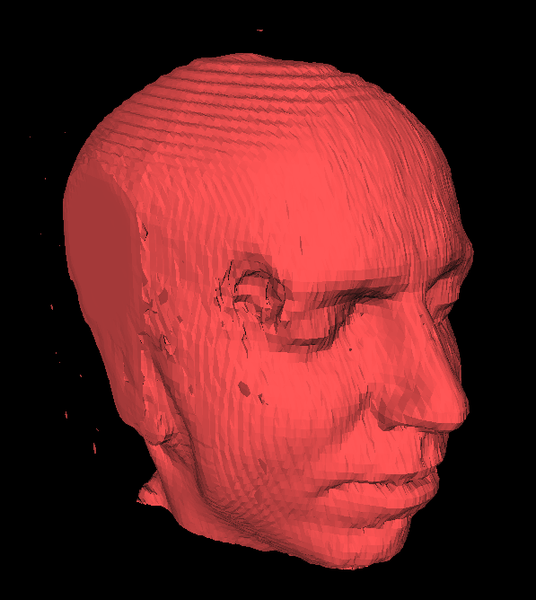
\includegraphics[width=6cm]{imagenes/marching_cubes_head}
		\caption{Cabeza extraída de 150 cortes obtenidos por una IRM usando \textit{marching cubes} (sobre 150.000 triángulos). Imagen extraída de \url{https://en.wikipedia.org/wiki/File:Marchingcubes-head.png}}
		\label{fig:marching_cubes_head}
	\end{figure}
	
	\item \textbf{Texturas 2D}: Se utilizan planos de corte alineados a los ejes de coordenadas. Por lo que se tendría una serie de cortes sobre el plano sagital, otra sobre el coronal y otra sobre el axial. Se realiza una interpolación bilineal para obtener la imagen final (Figura \ref{fig:texturas2d} \cite{intro_medical_vtk_bioimage}). Se puede usar en VTK con \texttt{vtkVolumeTextureMapper}.
	\begin{figure}[H]
		\centering
		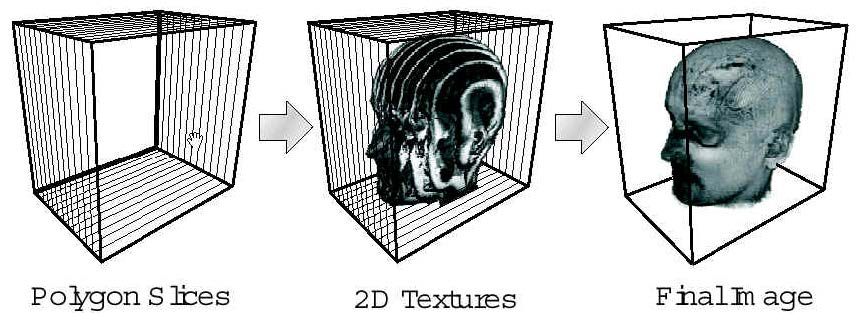
\includegraphics[width=10cm]{imagenes/texturas2d}
		\caption{Esquema del proceso de renderizado usando texturas 2D. Imagen extraída del apéndice B del libro \textit{An Introduction to Programming for Medical Image Analysis with the Visualization Toolkit }\cite{intro_medical_vtk_bioimage}}
		\label{fig:texturas2d}
	\end{figure}
	
	\item \textbf{Texturas 3D}: Esta técnica es similar a la anterior, pero ahora los datos se cargan en una textura 3D y los cortes se dibujan paralelos a la dirección de vista. A diferencia de las texturas 2D, usa interpolación trilineal y no es necesario tener almacenado en memoria tres copias de los mismos datos (Figura \ref{fig:texturas3d}) \cite{intro_medical_vtk_bioimage}. Se puede usar en VTK con \texttt{vtkVolumeTextureMapper3D}.
	\begin{figure}[H]
		\centering
		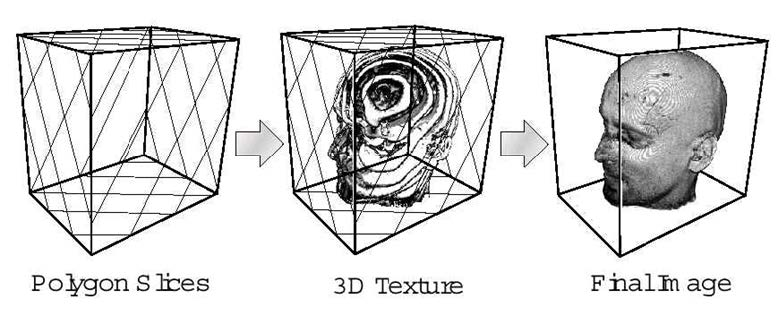
\includegraphics[width=10cm]{imagenes/texturas3d}
		\caption{Esquema del proceso de renderizado usando texturas 3D. Imagen extraída del apéndice B del libro \textit{An Introduction to Programming for Medical Image Analysis with the Visualization Toolkit} \cite{intro_medical_vtk_bioimage}}
		\label{fig:texturas3d}
	\end{figure}
	
	\item \textbf{\textit{Volume Ray Casting}}: Es una técnica en el que para cada pixel de la imagen se lanza un rayo que atraviesa el volumen. Para cada voxel se obtiene su color y opacidad usando una función de transferencia. Cuando el rayo sale del volumen se calcula el color y opacidad del pixel como el acumulado por el rayo. Existe una versión de este algoritmo que hace uso de la GPU para acelerar ostensiblemente el tiempo de la operación (Figura \ref{fig:volume_ray_casting}) \cite{intro_medical_vtk_bioimage}. Se puede usar en VTK con \texttt{vtkFixedVolumeRayCastMapper}, \texttt{vtkVolumeRayCastMapper} (usan CPU), \texttt{vtkGPUVolumeRayCastMapper} (usa GPU) y \texttt{vtkSmartVolumeMapper} (según el contexto usa CPU o GPU).
	\begin{figure}[H]
		\centering
		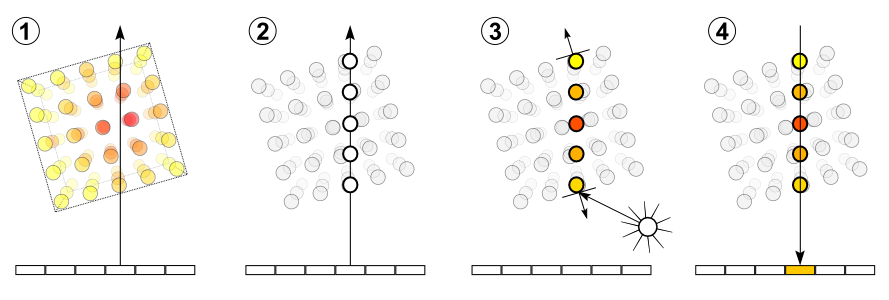
\includegraphics[width=12.5cm]{imagenes/volume_ray_casting}
		\caption{Esquema del proceso de \textit{ray casting}. Imagen extraída de \url{https://en.wikipedia.org/wiki/File:Volume_ray_casting.png}}
		\label{fig:volume_ray_casting}
	\end{figure}
\end{itemize}

De entre todas estas técnicas, se podrían descartar rápidamente la de \textit{marching cubes}: pues tan solo trabaja con isosuperficies, y la de texturas 2D: pues la opción de texturas 3D es más rápida y usa menos recursos. Sin embargo, la opción de \textit{marching cubes} será útil para poder crear una malla de triángulos que se pueda exportar a un formato con el que luego pueda ser imprimida en 3D.

Por tanto ya solo habría que elegir entre texturas 3D o \textit{ray casting}. Hasta hace unos años, VTK no proporcionaba un algoritmo de \textit{ray casting} que usase la GPU. Por tanto la opción habría sido sencilla, pero durante los últimos años han trabajado en esto haciendo del \textit{ray casting} la opción preferible.

\section{Volume Mapper}

Para poder visualizar un volumen con VTK mediante Direct Volume Rendering (DVR), necesitamos un \textit{Volume Mapper}. La librería nos ofrece varias alternativas:
\begin{itemize}
	\item \texttt{vtkAMRVolumeMapper}
	\item \texttt{vtkFixedVolumeRayCastMapper}
	\item \texttt{vtkGPUVolumeRayCastMapper}
	\item \texttt{vtkSmartVolumeMapper}
	\item \texttt{vtkVolumeRayCastMapper}
	\item \texttt{vtkVolumeTextureMapper}
	\item \texttt{vtkVolumeTextureMapper3D}
\end{itemize}

Entre esta lista tenemos algunos que utilizan o texturas o \textit{ray casting}, o la CPU o la GPU. Pero hay uno que es especial con respecto al resto. Se trata de \texttt{vtkSmartVolumeMapper}.

Este \textit{Volume Mapper} es una versión mejorada del \texttt{vtkGPUVolumeRayCast Mapper} por lo que utiliza la GPU (si el dispositivo cuenta con una) y la técnica de \textit{ray casting}. Además cuenta con nuevas características con respecto al resto, como el poder definir infinitos planos de corte para poder ver el interior del volumen \cite{smart_volume_mapper}.

Por tanto, el \textit{Volume Mapper} utilizado será el \texttt{vtkSmartVolumeMapper}.

\section{Función de transferencia}

La función de transferencia es la encargada de dar a un valor de intensidad las propiedades de color y opacidad que le corresponden para la visualización del volumen.

En VTK la función de transferencia forma parte de la clase \texttt{vtkVolume Property} \cite{vtk_example_medical4}. Para ello proporciona otras dos clases:
\begin{itemize}
	\item \texttt{vtkColorTransferFunction}: Para definir el color. Se enlaza a \texttt{vtk VolumeProperty} con el método \texttt{SetColor}.
	\item \texttt{vtkPiecewiseFunction}: Para definir la opacidad (tanto escalar como gradiente). La opacidad escalar se enlaza a \texttt{vtkVolumeProperty} con el método \texttt{SetScalarOpacity} y la gradiente con \texttt{SetGradientOpacity}.
\end{itemize}

Podemos, por tanto, diferenciar tres partes fundamentales en la función de transferencia, la encargada de dar la propiedad de color y las dos de dar la propiedad de opacidad. Ambas trabajan de forma independiente. Es decir, cuando se define un punto en una de ellas, no tiene por qué definirse en la otra.

\subsection{Color}

Para definir esta función (\texttt{vtkColorTransferFunction}), hay que agregar puntos para valores de intensidad a los que se les asignará un color. VTK se encargará de interpolar entre un punto y otro (Figura \ref{fig:color_tf}). 

Por defecto, cuando no hay ningún punto, a todos los valores de intensidad les corresponderá un color negro. De forma parecida se comporta cuando solo hay un punto pero en lugar de negro, les corresponderá el color del punto que se ha definido.

VTK permite trabajar tanto con HSV como con RGB y para añadir un punto hay que utilizar \texttt{AddHSVPoint} o \texttt{AddRGBPoint}. A estos métodos se les pasa un primer parámetro en coma flotante con el valor de intensidad donde se establecerá ese punto y otros tres con las distintas exponentes (\textit{hue}, \textit{saturation}, \textit{brightness} o \textit{red}, \textit{green}, \textit{blue}).

\begin{figure}[H]
	\centering
	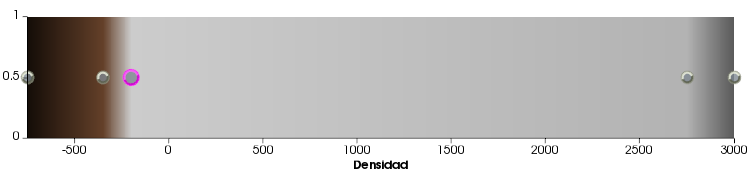
\includegraphics[width=12.5cm]{imagenes/color_tf}
	\caption{Parte de color de la función de transferencia del \textit{preset} \textit{CT-WoodSculpture} creado para visualizar esculturas de madera policromadas. Dos puntos definen el color. Uno en -750 con un tono más oscuro y otro en -350 con un tono más claro. El estuco se pinta con un color gris claro y también viene definido por dos puntos: -200 y 2750. Finalmente, el metal se verá con un tono gris oscuro definido con un punto en 3000.}
	\label{fig:color_tf}
\end{figure}

\subsection{Opacidad}

El valor de opacidad se obtendría como el \textbf{producto de la opacidad escalar por la gradiente}. Si no se define alguna de las dos, se definiría como un valor constante de 1 para que solo se viese el resultado de la que sí está definida.

\subsubsection{Opacidad escalar}

Con el color no bastaría, pues si comprobásemos ahora añadiéndole tan solo el \texttt{vtkColorTransferFunction} al \texttt{vtkVolumeProperty} observaríamos que no se pinta nada en pantalla. Esto es porque por defecto, al no tener ningún punto la función de opacidad (\texttt{vtkPiecewiseFunction}) es una constante con valor 0 (transparente). 

Para definir esta función se trabaja de forma parecida a como se hace con el color, añadiendo puntos. El método que hay que utilizar es \texttt{AddPoint} al que se le pasan dos parámetros en coma flotante. El primero con el valor de intensidad y el segundo con la opacidad en ese punto. Para obtener los valores en puntos intermedios, se interpola entre los dos puntos en los que está. De forma que si para el valor de intensidad 100 hemos definido una opacidad de 0.5 y para el de 200 1, al valor de intensidad 150 le corresponderá 0.75.

Combinando color y opacidad escalar podemos obtener una función de transferencia para visualizar nuestro volumen (Figura \ref{fig:opacity_tf}), pero para obtener mejores resultados, habrá que utilizar la opacidad gradiente. 

\begin{figure}[H]
	\centering
	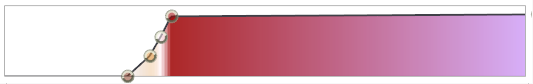
\includegraphics[width=12.5cm]{imagenes/opacity_tf}
	\caption{Parte de opacidad escalar de la función de transferencia del \textit{preset} \textit{CT-WoodSculpture} creado para visualizar esculturas de madera policromadas. Se pueden observar tres regiones. La primera corresponde a la madera, la segunda al estuco y la última al metal}
	\label{fig:opacity_tf}
\end{figure}

\subsubsection{Opacidad gradiente}

La opacidad gradiente utiliza el vector gradiente para dar el valor de opacidad. Con éste se puede conseguir \textbf{dar un mayor valor a regiones de los bordes, así como menor a regiones planas} es decir, donde no varía el valor de intensidad de sus vecinos de alrededor.

El gradiente se mide como la cantidad que varía la intensidad en una unidad de distancia. Este cálculo del gradiente lo realiza VTK cuando genera el volumen de forma transparente sin que haya que añadir nada al código.

Para poder definir la función de la opacidad gradiente, al igual que con las demás, hay que añadir puntos con la misma función que se usaba con la opacidad escalar (\texttt{AddPoint}). 

\begin{figure}[H]
	\centering
	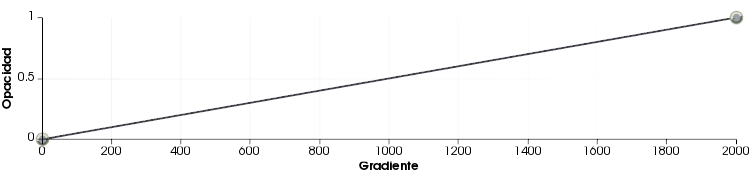
\includegraphics[width=12.5cm]{imagenes/gradient_tf}
	\caption{Parte de opacidad gradiente de la función de transferencia del \textit{preset} \textit{CT-WoodSculpture} creado para visualizar esculturas de madera policromadas. Se obtendría un valor cercano a 1 en la opacidad en aquellas zonas más cercanas a los bordes entre materiales pues se ha establecido que para un gradiente 0 la opacidad sea 0, y para 2000, 1. }
	\label{fig:gradient_tf}
\end{figure}

\section{Escala Hounsfield}

Como ya se ha explicado, para desarrollar la función de transferencia con la que se visualiza el volumen, juega un papel muy importante el valor de densidad del material. 

Este valor se encuentra en unas unidades conocidas como Unidades Hounsfield (HU) en honor al ingeniero Godfrey Newbold Hounsfield, inventor del primer escáner TAC con el que ganó el Premio Nobel de Fisiología o Medicina en 1979.

La Escala Hounsfield no es más que la transformación de la escala de coeficientes de atenuación lineal de rayos X a una nueva en relación al valor del agua destilada en condiciones normales de presión y temperatura.

El valor de HU de un material viene dado por la siguiente fórmula:

\[ HU = 1000 \times \frac{\mu_{mat}-\mu_{agua}}{\mu_{agua}} \]

Donde $ \mu_{mat} $ es el coeficiente de atenuación lineal del material y $ \mu_{agua} $ el del agua.

Por tanto, el valor teórico del agua será 0 HU.

El rango de valores de la escala va desde -1024 HU hasta 3071 HU. 4096 valores representados mediante 12 bits.

\begin{table}[H]
	\begin{center}
		\begin{tabular} {|l|l|}
			\hline
			Material & HU \\ \hline
			\hline
			Aire & -1000 \\ \hline
			Madera & -750 a -350 \\ \hline
			Estuco & 200 a 1000 \\ \hline
			Metal & 2900 a 3000 \\ \hline
		\end{tabular}
		\caption{Valores en HU de distintos materiales presentes en imágenes de esculturas de madera}
		\label{tab:materials_hu}
	\end{center}
\end{table}